%\documentclass[manuscript]{aastex}
%\documentclass[numberedappendix]{emulateapj}

%\documentclass[12pt,titlepage,preprint]{aastex}
%\documentclass{article}
\documentclass[preview,multi=singlepage,border=3pt]{standalone}
%\bibliographystyle{../_demoResources/configs/zhihu/apj}
\bibliographystyle{ieeetr}
\usepackage[square,comma,numbers,sort&compress]{natbib}

\usepackage{color}\definecolor{RED}{rgb}{1,0,0}\definecolor{BLUE}{rgb}{0,0,1} %DIF PREAMBLE
\usepackage{ulem}
\usepackage{float}
\usepackage[caption = false]{subfig}
\usepackage{graphicx}
\usepackage{multirow}
\usepackage{mathtools}
\usepackage{afterpage}
\usepackage{emptypage}
\usepackage{pdflscape}
\usepackage{rotating}
%\usepackage{url}
\usepackage{geometry}
\usepackage{tabulary}
\usepackage{booktabs}

\usepackage{rotating}
\usepackage{comment}

\usepackage{amsmath}
\usepackage{fontenc}
\usepackage[UTF8]{ctex}

\usepackage{fontspec}
\newfontfamily\zhfont[BoldFont=Adobe Heiti Std]{Adobe Song Std}
\newfontfamily\zhpunctfont{Adobe Song Std}
\setmainfont{Times New Roman}

\usepackage[colorlinks,linkcolor={}]{hyperref}

\pagenumbering{gobble}
\usepackage{stackengine}
\stackMath

%\usepackage[active,floats,tightpage]{preview}
%\setlength\PreviewBorder{5pt}%

%\newcommand{\Newpage}{\end{preview}\begin{preview}}
%\newcommand\arcsec{\mbox{$^{\prime\prime}$}}
\newcommand{\angstrom}{{\rm \AA}}

\newcommand{\etal}{et al.}
\newcommand{\hbeta}{H{$\beta$}}
\newcommand{\halpha}{H{$\alpha$}}
\newcommand{\hdelta}{H{$\delta_{{\rm A}}$}}
\newcommand{\CIV}{C{\sevenrm\,IV}}
\newcommand{\SiIV}{Si{\sevenrm\,IV}}
\newcommand{\CIII}{C{\sevenrm\,III]}}
\newcommand{\MgII}{Mg{\sevenrm\,II}}
\newcommand{\MgIIb}{Mg{\sevenrm\,II}\,$\lambda$2800}
\newcommand{\OIV}{O{\sevenrm\,IV}}
\newcommand{\OIII}{[O{\sevenrm\,III}]}
\newcommand{\loiii}{$L_{\text{[O \textrm{\tiny III}]}}$}
\newcommand{\OIIIa}{[O{\sevenrm\,III}]\,$\lambda$4959}
\newcommand{\OIIIb}{[O{\sevenrm\,III}]\,$\lambda$5007}
\newcommand{\OIIIc}{[O{\sevenrm\,III}]\,$\lambda\lambda$4959,5007}
\newcommand{\NII}{[N{\sevenrm\,II}]}
\newcommand{\NIIb}{[N{\sevenrm\,II}]\,$\lambda$6584}
\newcommand{\SII}{[S{\sevenrm\,II}]}
\newcommand{\SIIa}{[S{\sevenrm\,II}]\,$\lambda$6717}
\newcommand{\SIIb}{[S{\sevenrm\,II}]\,$\lambda$6731}
\newcommand{\SIIab}{[S{\sevenrm\,II}]\,$\lambda\lambda$6717,6731}
\newcommand{\lgL}{\log \, \left({L_{\rm bol} \over {\rm erg\,s^{-1}}}\right)}
\newcommand{\bracket}[1]{\left\langle#1\right\rangle}
\font\bften=cmbx10 scaled 1000 \font\tenrm=cmr10 scaled 1000
\font\eightrm=cmr8 scaled 1000 \font\sevenrm=cmr7 scaled 1000

\newcommand{\lya}{$\rm{Ly}\alpha$ }
\newcommand{\lyb}{$\rm{Ly}\beta$ }
\newcommand{\A}{{\rm \AA} }

\def\chandra{{\it Chandra}}
\def\xmmnewton{{\it XMM-Newton}}
\def\swift{{\it Swift}}
\def\hst{{\it HST}}
\def\galfit{{\tt GALFIT}}
\def\sersic{S\'{e}rsic}
\newcommand{\mpsf}{$m_{\rm P}$}
\newcommand{\mser}{$m_{\rm S}$}
\newcommand{\reff}{$R_{\rm e}$}
\newcommand{\loiiiOBS}{$L^{\rm obs}_\text{[{\scriptsize O} \textrm{\tiny III}]}$}
\newcommand{\loiiiCOR}{$L^{\rm cor}_\text{[{\scriptsize O} \textrm{\tiny III}]}$}
\newcommand{\lbol}{$L_{\rm bol}$}
\newcommand{\REdd}{$\lambda_\mathrm{Edd}$}
\newcommand{\cgs}{ ${\rm erg~cm}^{-2}~{\rm s}^{-1}$}
\newcommand{\lum}{(\rm erg~s$^{-1}$)}
\newcommand{\rpy}{$r_{\mathrm{p}, Y}$}

\renewcommand{\le}{$<$ }
\newcommand{\araa}{ARAA}
\newcommand{\apjl}{APJL}
\newcommand{\aap}{AAP}

\renewcommand\equationautorefname{Eq. }
\renewcommand\subsectionautorefname{\S}
\renewcommand\sectionautorefname{\S}


%\renewcommand{\thesection}{}
%\renewcommand{\thesubsection}{}
%\renewcommand{\thesubsection}{{section}.{subsection}}
\makeatletter
\def\@seccntformat#1{\csname #1ignore\expandafter\endcsname\csname \endcsname\quad}
\let\sectionignore\@gobbletwo
\let\latex@numberline\numberline
\def\numberline#1{\if\relax#1\relax\else\latex@numberline{#1}\fi}
\makeatother

\makeatletter
\def\@subseccntformat#1{\csname #1ignore\expandafter\endcsname\csname \endcsname\quad}
\let\subsectionignore\@gobbletwo
\let\latex@numberline\numberline
\def\numberline#1{\if\relax#1\relax\else\latex@numberline{#1}\fi}
\makeatother

\newcommand{\newsinglepage}{\end{singlepage}\begin{singlepage}}


% some improvement for scriv
\renewcommand{\[}{\begin{equation}} 
\renewcommand{\]}{\end{equation}} 
%\renewcommand{\citet}{\citealt}

\begin{document}
\begin{singlepage}


%  Comments:
%  * Choose which bibliography file to include in the  ../configs/SimpleOneColumn/footer.tex
%  Mind the path in all the included .tex file


%Make sure that 
    %* You select the parent folder (“SimpleOneColumn” in this example) as the Compile Group
    %* The “Treat compile group as entire draft” options is checked
    %* the “Article” is included
%
% Make a folder that have the same name as your .tex file (if the folder does not exists, you need do this only once)
% Because we want to make the root folder clean (as latex will generate lots of temp file when compile)
%
% Click Replace here, and finish export
%



% use \newsinglepage to generate another page


\section{Introduction 简介}
\label{sec:intro}

\subsection{Test for cite and enumerate and term 同时测试中文}
\label{sec:cite}

Test for cite and enumerate %some comments

% Some comments


% Without ";", citep
% With ";", citet


Example:

\begin{verbatim}
[#Kormendy&Ho2013ARA&A, Koss2012ApJ]
[#Kormendy&Ho2013ARA&A, Koss2012ApJ][]
[foo][#Kormendy&Ho2013ARA&A, Koss2012ApJ]
[foo\]\[bar][#Kormendy&Ho2013ARA&A, Koss2012ApJ]

[#Kormendy&Ho2013ARA&A, Koss2012ApJ;]
[#Kormendy&Ho2013ARA&A, Koss2012ApJ;][]
[foo][#Kormendy&Ho2013ARA&A, Koss2012ApJ;]
[foo\]\[bar][#Kormendy&Ho2013ARA&A, Koss2012ApJ;]
\end{verbatim}

Term:

\begin{itemize}
\item ~\citep{Kormendy&Ho2013ARA&A, Koss2012ApJ}

\begin{itemize}
\item ~\citep{Kormendy&Ho2013ARA&A, Koss2012ApJ}

\end{itemize}

\item ~\citep[foo]{Kormendy&Ho2013ARA&A, Koss2012ApJ}

\begin{itemize}
\item ~\citep[foo][bar]{Kormendy&Ho2013ARA&A, Koss2012ApJ}

\end{itemize}

\end{itemize}

Enumerate:

\begin{enumerate}
\item  \citet{Kormendy&Ho2013ARA&A, Koss2012ApJ}

\item  \citet{Kormendy&Ho2013ARA&A, Koss2012ApJ}

\item  \citet[foo]{Kormendy&Ho2013ARA&A, Koss2012ApJ}

\item  \citet[foo][bar]{Kormendy&Ho2013ARA&A, Koss2012ApJ}

\end{enumerate}

Here is not cited(~\nocite{Povic2012A&A}).

Here is a enumerate:

\begin{enumerate}
\item Type for ``1984.''

\end{enumerate}

Here is not:

1984. Type for ``1984.''

List of Markers:

\textbackslash{} Backslash0
\textbackslash{} Backslash1

\texttt{Backtick0
} Backtick1

\begin{itemize}
\item Asterisk0

\item Asterisk1

\item plus sign0

\item plus sign1

\item minus sign0 (hyphen)

\item minus sign1 (hyphen)

\end{itemize}

This is a line.
This is a new line.

Cite for intro \S\nameref{sec:intro}

Cite for cite note (\autoref{sec:cite})

Cite for quote \S\nameref{sec:quote}

在这里测试中文的显示效果

\subsection{Test for quote}
\label{sec:quote}

Test for quote:

\begin{quote}

Level 1
Lazy type in for level 1

Level 1, must have a empty line for new line,
Level 1 (failed new line)

\begin{quote}

Level 2
Lazy type in for level 2, must have a empty type for lazy type

Level 2

Level 2 (successful new line)

\begin{quote}

Level 3
Lazy type in for level 3,
 Not lazy type in for level 3
\end{quote}
\end{quote}
\end{quote}

\newsinglepage

\section{Other test}
\label{set:other}

\subsection{test for rules}
\label{testforrules}

Test for rules:

Some

\begin{center}\rule{3in}{0.4pt}\end{center}


Thing

\begin{center}\rule{3in}{0.4pt}\end{center}


Between

\begin{center}\rule{3in}{0.4pt}\end{center}


different 

\begin{center}\rule{3in}{0.4pt}\end{center}


rules

\begin{center}\rule{3in}{0.4pt}\end{center}


En{\ldots}

\subsection{test for Links}
\label{testforlinks}

This is \href{http://example.com/}{an example}\footnote{\href{http://example.com/}{http:/\slash example.com\slash }} inline link.

\href{http://example.net/}{This link}\footnote{\href{http://example.net/}{http:/\slash example.net\slash }} has no title attribute.

Also we can add a foot note\footnote{http:\slash \slash example.net\slash }

Or like \href{http://example.com}{this}\footnote{\href{http://example.com}{http:/\slash example.com}}

Or like \href{http://example.com}{id}\footnote{\href{http://example.com}{http:/\slash example.com}}

I get 10 times more traffic from \href{http://google.com/}{Google}\footnote{\href{http://google.com/}{http:/\slash google.com\slash }} than from
\href{http://search.yahoo.com/}{Yahoo}\footnote{\href{http://search.yahoo.com/}{http:/\slash search.yahoo.com\slash }} or \href{http://search.msn.com/}{MSN}\footnote{\href{http://search.msn.com/}{http:/\slash search.msn.com\slash }}.

\subsection{test for emphasis}
\label{testforemphasis}

\emph{single asterisks}

\emph{single underscores}

\textbf{double asterisks}

\textbf{double underscores}

*this text is surrounded by literal asterisks*

\subsection{test for code}
\label{testforcode}

Use the \texttt{printf()} function.

\texttt{There is a literal backtick (`) here.}

A single backtick in a code span: \texttt{`}

A backtick-delimited string in a code span: \texttt{`foo`}

Please don't use any \texttt{$<$blink$>$} tags.

\texttt{\&\#8212;} is the decimal-encoded equivalent of \texttt{\&mdash;}.

\subsection{test for equation}
\label{testforequation}

Some equations: eq:0 (\autoref{eq:0})

$${x}_{1,2} = \frac{-b\pm \sqrt{{b}^2}-4ac}{2a} \label{eq:0}$$ %equation with no equation number

\[{x}_{1,2} = \frac{-b\pm \sqrt{{b}^2}-4ac}{2a} \label{eq:5} \] %equation with equation number

Inline: ${x}_{1,2} = \frac{-b\pm \sqrt{{b}^2}-4ac}{2a}$ , blabla

Inline: ${x}_{1,2} = \frac{-b\pm \sqrt{{b}^2}-4ac}{2a}\label{eq:3}$ , blabla

公式堆叠测试
\[
\setstackgap{S}{2pt}
\stackunder{\stackon{\text{text}}{\scriptstyle i=n}}{\scriptstyle i=1}
\quad
\underset{\textrm{下面}}{\overset{\textrm{上面}}{\text{text}}}
\]

eq:1 (\autoref{eq:5}) eq3 inline (\autoref{eq:3})
 % This figure will not include in the final test
% Any thing in the comment region will be inserted directly into the output .tex file

\begin{equation}
1=\Omega_0+\underset{\textrm{暗能量}}{\overset{\textrm{这是}}{\Omega_{\Lambda}}}+\Omega_k, \label{eq:1}
\end{equation}
And:
\begin{eqnarray}
&\Omega_0=\frac{\rho_0}{\rho_{c0}}=\Omega_m+\Omega_r; \\
&\Omega_{\Lambda}=\frac{\rho_{\Lambda}}{\rho_{c0}}; \\
&\Omega_k=-\frac{kc^2}{a_0^2H_0^2}; \label{eq:2}
\end{eqnarray}


\subsection{test for table}
\label{testfortable}

MultiMarkdown table here (\autoref{table:multimarkdown}): 

\begin{table}[htbp]
\begin{minipage}{\linewidth}
\setlength{\tymax}{0.5\linewidth}
\centering
\small
\caption{Very very very very very very very very very long caption}
\label{table:multimarkdown}
\begin{tabulary}{\textwidth}{@{}LCR@{}} \toprule
&Grouping&\\
First Header&Second Header&Third Header\\
\midrule
Content&\emph{Long Cell}&\\
Content&\textbf{Cell}&Cell\\

\midrule
New section&More&Data\\
And more&And more&\\

\bottomrule

\end{tabulary}
\end{minipage}
\end{table}

Large Table:large (\autoref{table:large})


\begin{table*}
\caption{Photometric Parameters}
\begin{center}
\begin{tabular}{c c c c c c c c c}
  \hline
  \hline
  Target name     & Aperture & $m_Y$           & $m_U$           & $M_z$  & $M_u$  & $u-z$          & $M_*$ & B/T  \\ 
      (1)         &    (2)   &  (3)            &  (4)            &   (5)  &   (6)  &  (7)           &  (8)  & (9)  \\ \hline
SDSS J1108+0659   & $18''$   & 16.24$\pm 0.05$ & 18.48$\pm 0.26$ & -23.12 & -21.37 & 1.76$\pm 0.26$ & 11.14 & 0.55 \\
SDSS J1131$-$0204 & $12''$   & 15.81$\pm 0.01$ & 18.94$\pm 0.09$ & -23.04 & -20.39 & 2.65$\pm 0.10$ & 11.24 & 0.12 \\
SDSS J1146+5110   & $18''$   & 15.89$\pm 0.03$ & 18.40$\pm 0.14$ & -22.68 & -20.65 & 2.02$\pm 0.14$ & 11.00 & 0.41 \\
SDSS J1332+0606   & $12''$   & 16.82$\pm 0.04$ & 19.29$\pm 0.16$ & -22.86 & -20.88 & 1.98$\pm 0.17$ & 11.07 & 0.69 \\ \hline
\end{tabular}
Col. 2: the aperture sizes that are large enough to enclose more than $95\%$ flux of the galaxies; 
Col. 3 \& 4: the apparent magnitudes in $Y$ and $U$ bands measured with the apertures correspondingly. 
The uncertainties are estimated from 1 $\sigma$ variation of the sky background; 
Col. 5 \& 6: the SDSS $z$- and $u$-band absolute magnitudes of the targets, transformed from $m_Y$ and $m_U$ correspondingly, assuming a flat local spectra ($f_{\lambda} \sim const.$) around the relevant frequencies; 
Col. 7: color calculated from the $u$ and $z$ magnitudes; 
Col. 8: the stellar mass in solar unit of the targets estimated from the $z$- and $u$-band magnitudes (see the text for details, \S \ref{subsec:mass}). 
Col. 9: the bulge-to-total mass ratios. 
The bulge mass is obtained by adding up the two bulge components in \galfit\ decomposition results for each galaxy.                                                         
\end{center}

\label{table:large}
\end{table*}%

\newsinglepage

\section{Test for figs}
\label{testforfigs}


%Use 
%   ![caption][label]
%   And later
%   [label]: $PATH width="0.30\textwidth" height="0.25\textheight"



Include some figure:

Image one (image with given size, 200x400): image fixed (\autoref{image:small})

\begin{figure}[htbp]
\centering
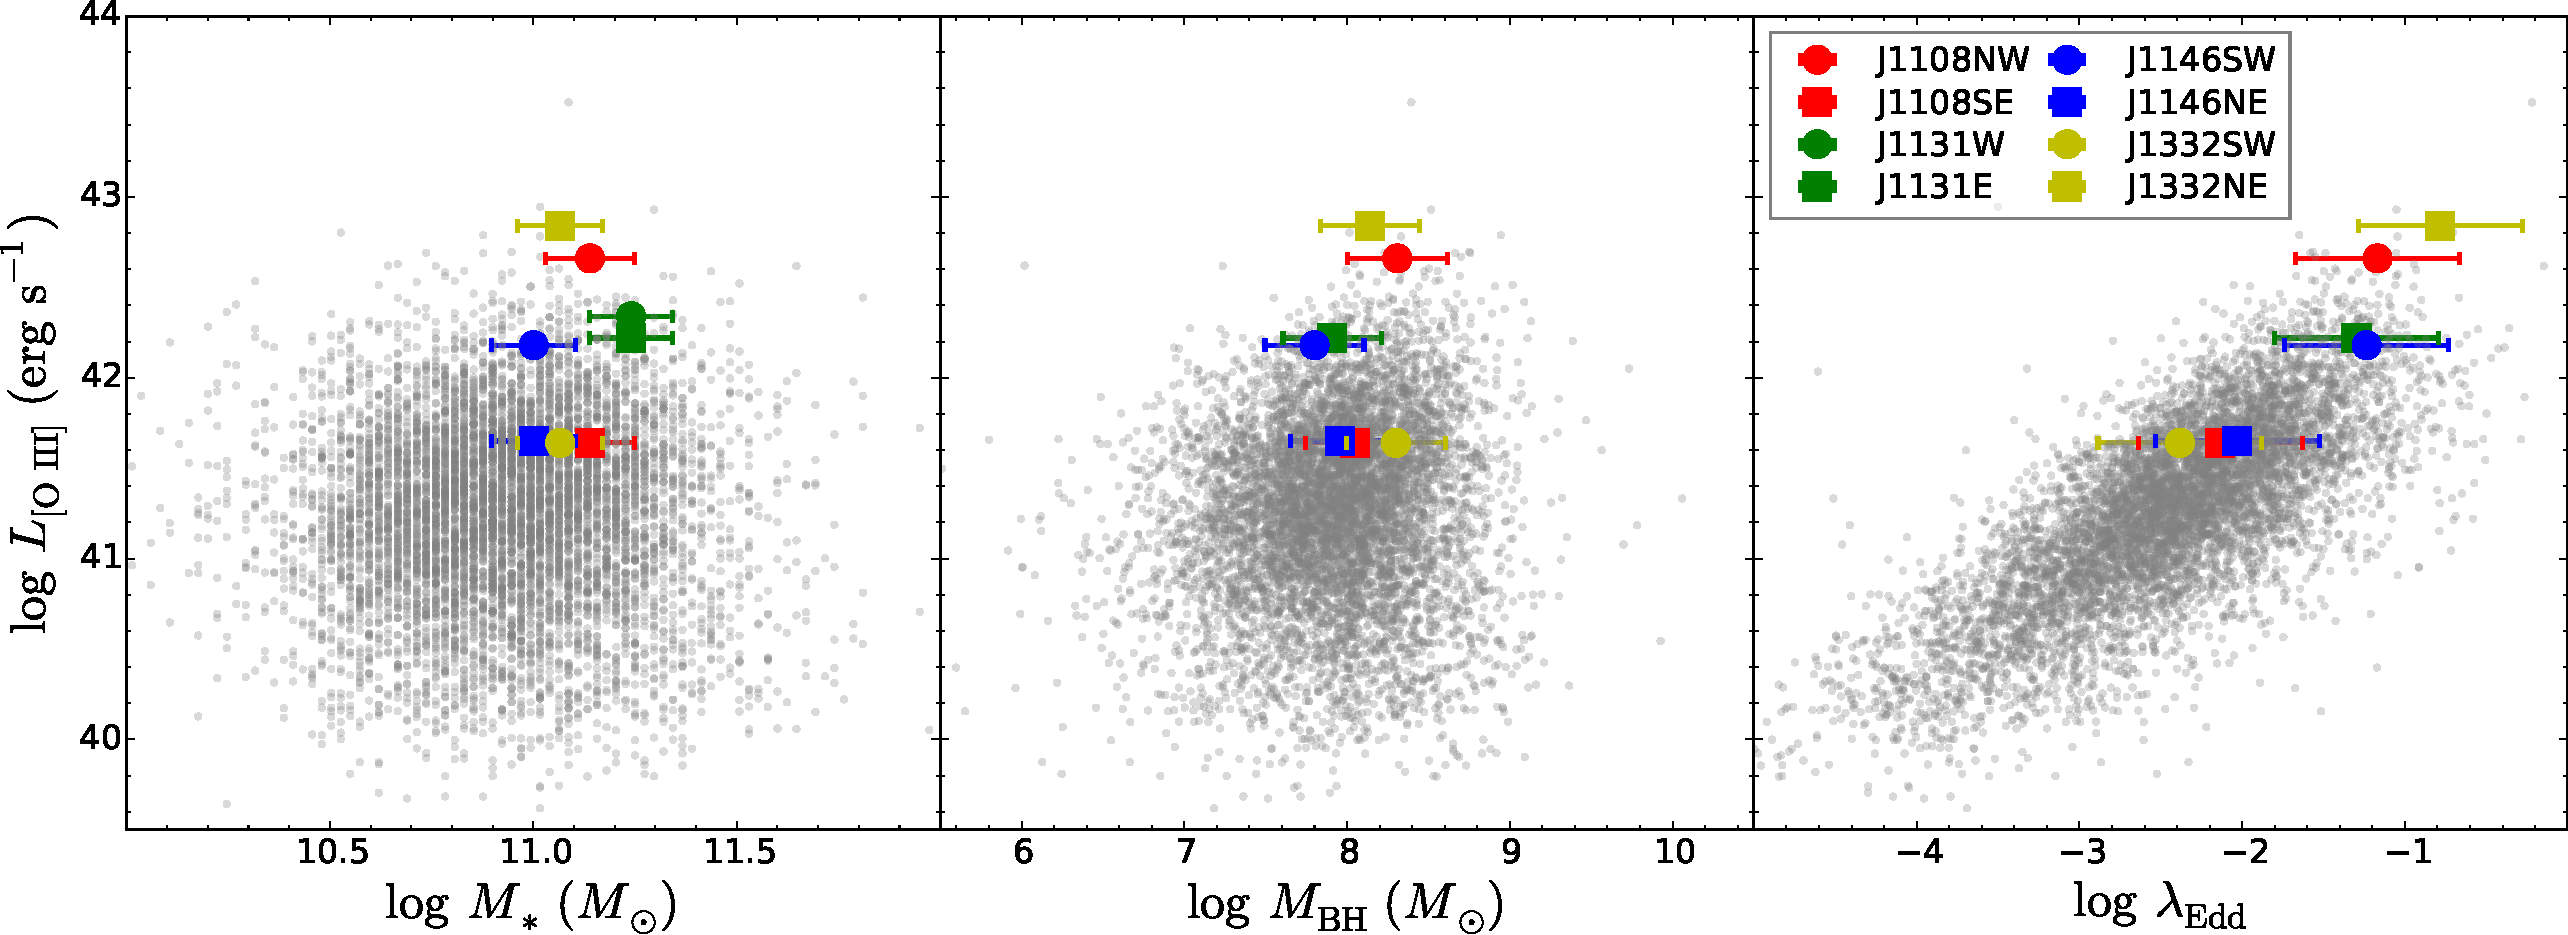
\includegraphics[width=300pt,height=200pt]{../_demoResources/figs/zhihu/comp_dr7.pdf}
\caption{Fig with give size, 200x400}
\label{image:fixed}
\end{figure}

Image two (image direct): image direct, no way to ref it (\autoref{image:direct})

\begin{figure}[htbp]
\centering
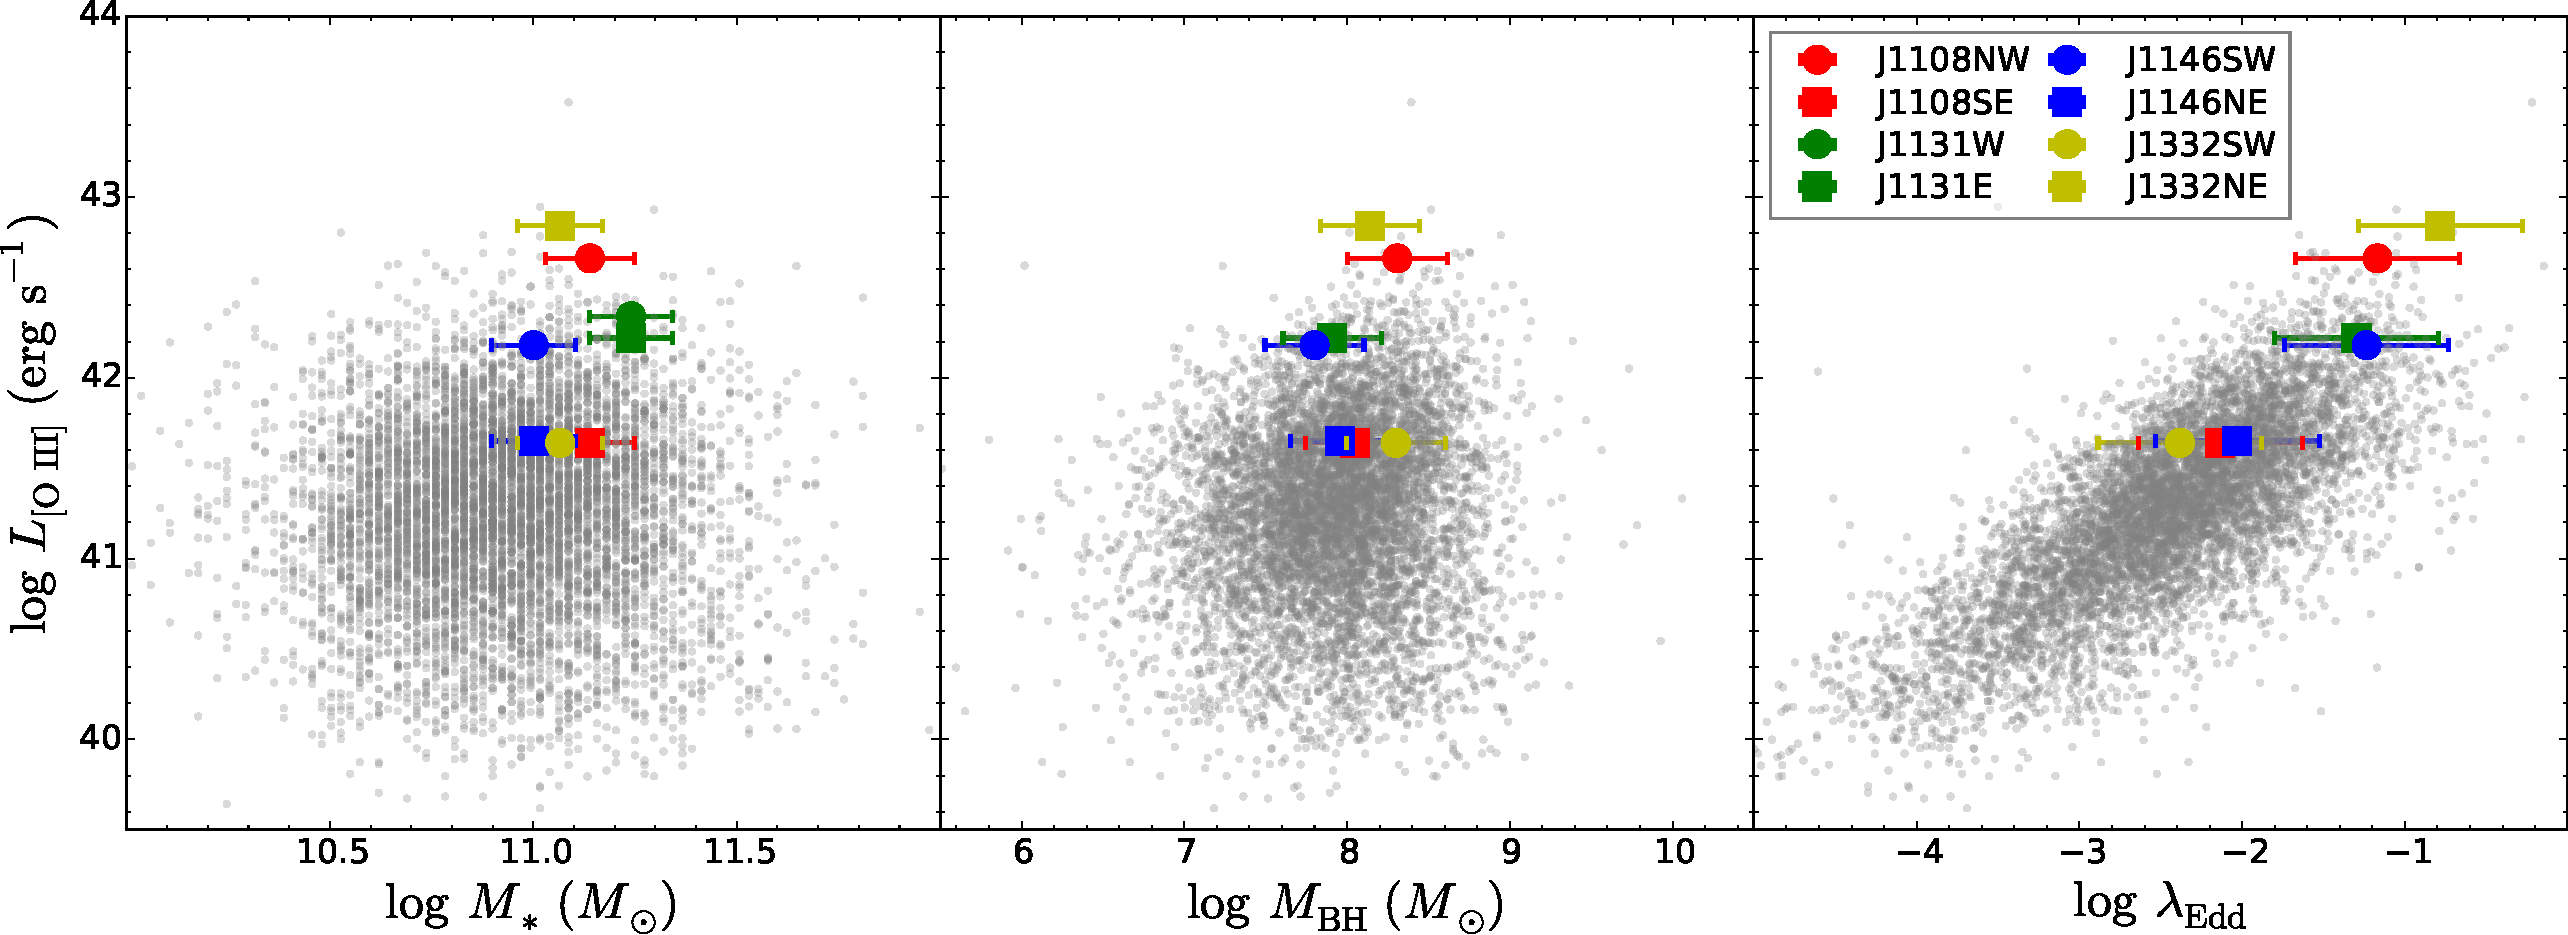
\includegraphics[keepaspectratio,width=\textwidth,height=0.75\textheight]{../_demoResources/figs/zhihu/comp_dr7.pdf}
\caption{Direct figure title}
\end{figure}

Image three (image: normal): \autoref{image:normal}

\begin{figure}[htbp]
\centering
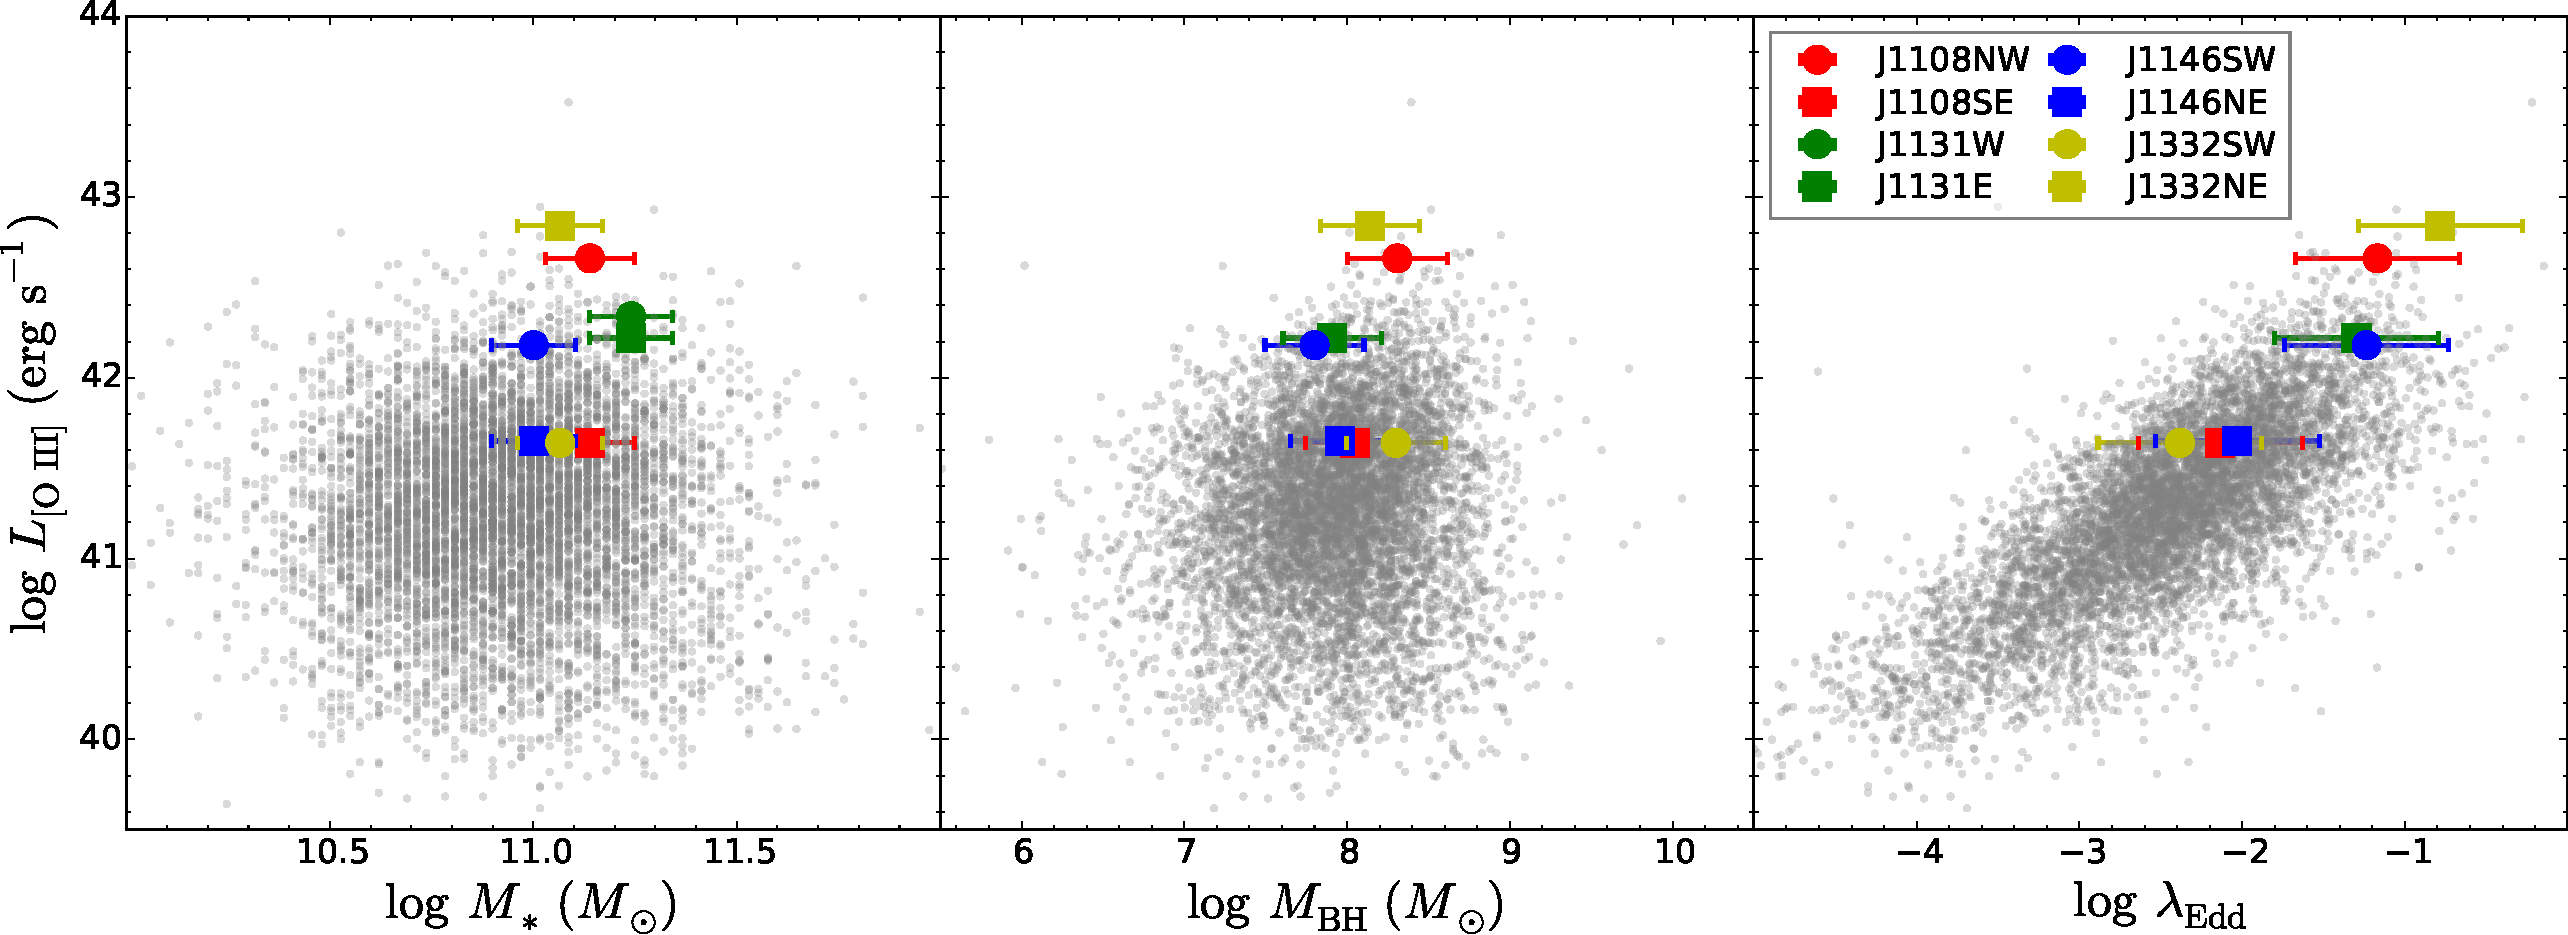
\includegraphics[keepaspectratio,width=\textwidth,height=0.75\textheight]{../_demoResources/figs/zhihu/comp_dr7.pdf}
\caption{Here we have our long long blablaFigblablaFigblablaFigblabla FigtitleblablaFigblablaF igblablaFigblablaFigti tleblablaFigblablaFig, \small A demonstration of our near- to far-IR SEDs of PG quasars, produced by \cite{Kormendy&Richstone1995ARA&A}., I try to ref intro (\autoref{sec:intro})}
\label{image:normal}
\end{figure}

Image Four (image:small):\autoref{image:small}

\begin{figure}[htbp]
\centering
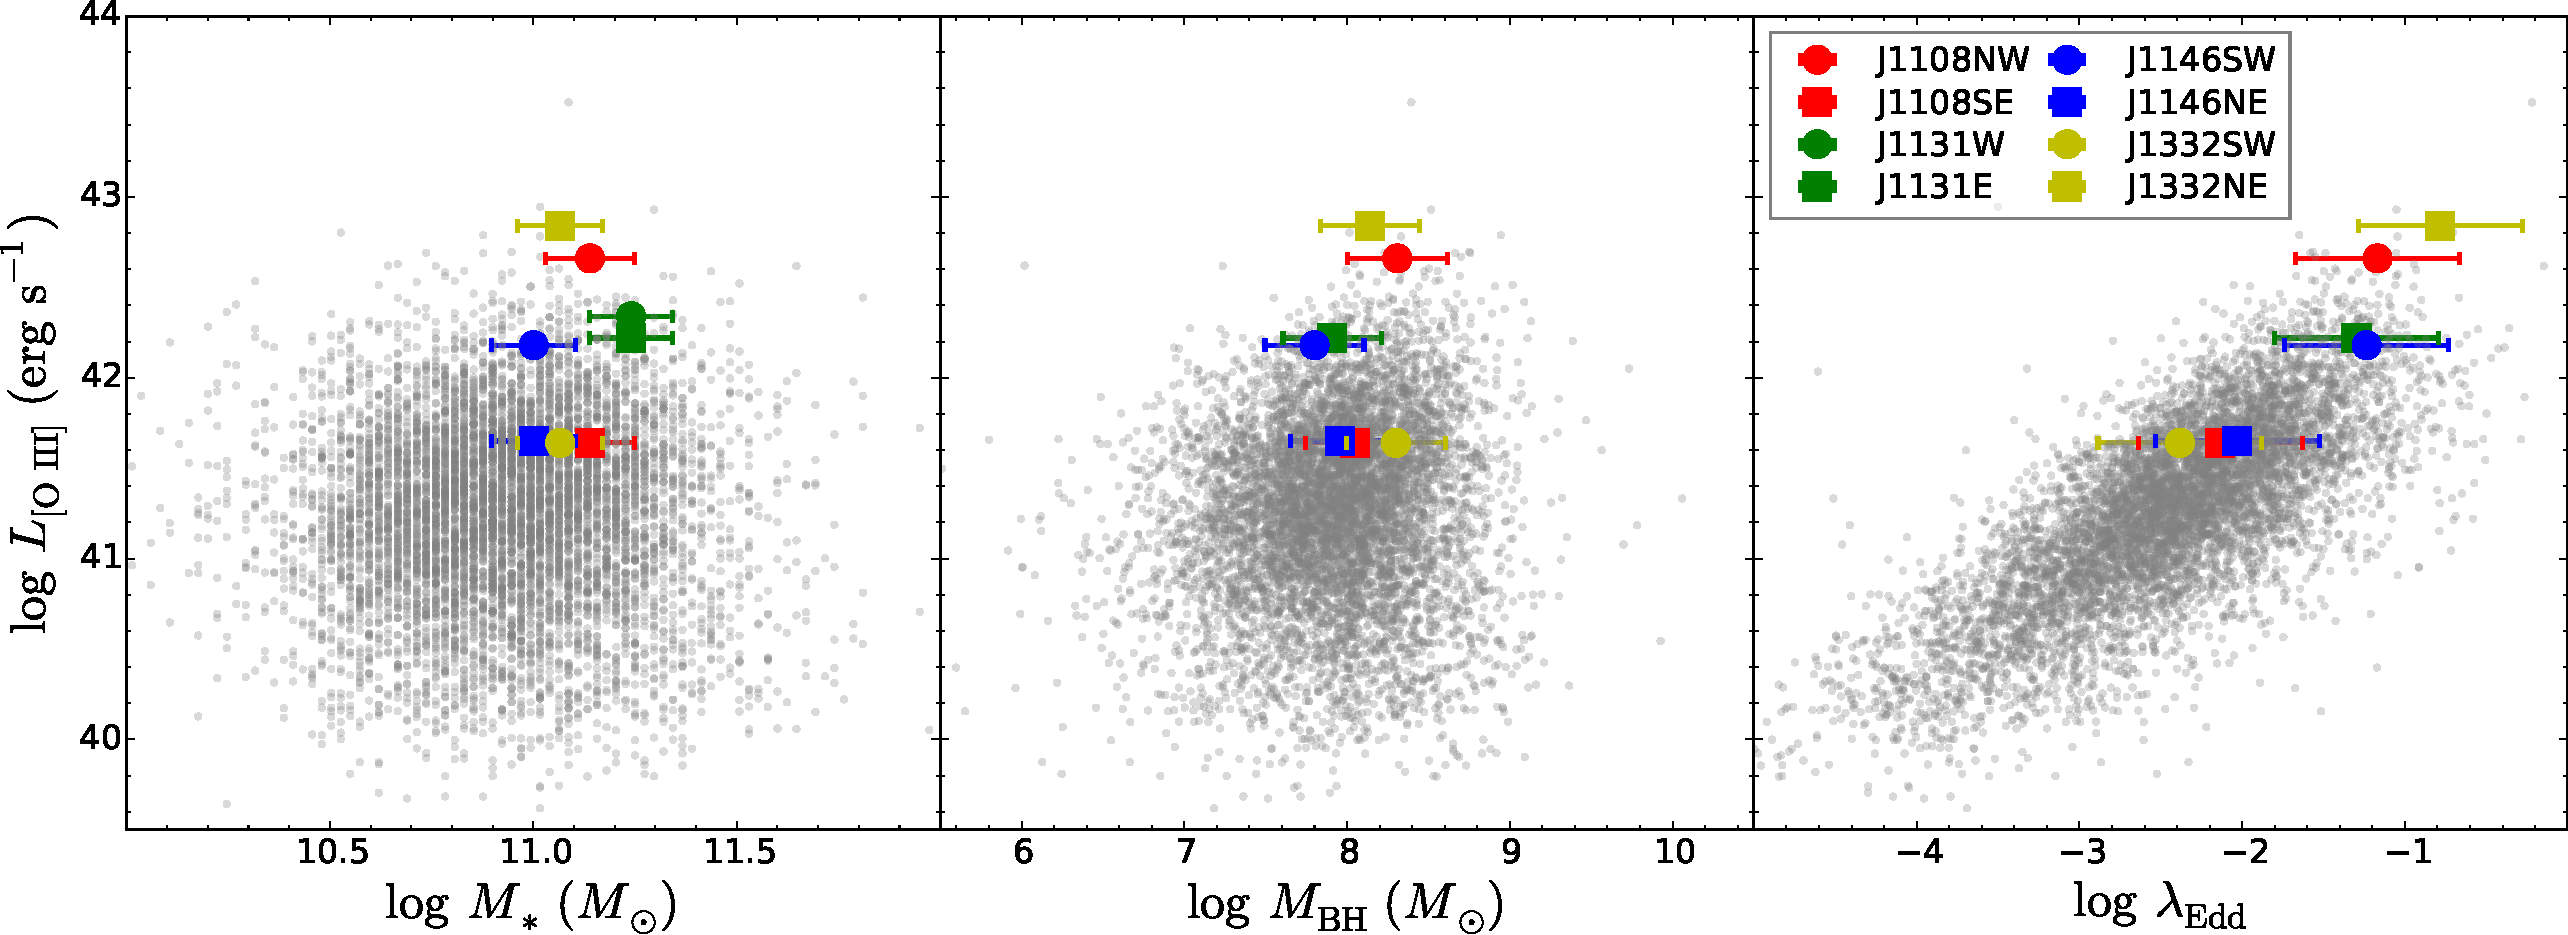
\includegraphics[width=0.30\textwidth,height=0.25\textheight]{../_demoResources/figs/zhihu/comp_dr7.pdf}
\caption{0.3 \textbackslash{}textwidth and 0.25 \textbackslash{}textheight, compare the size with \autoref{image:normal}}
\label{image:small}
\end{figure}

Good include: cmp (\autoref{fig:cmp})


\begin{figure*}
\begin{center}
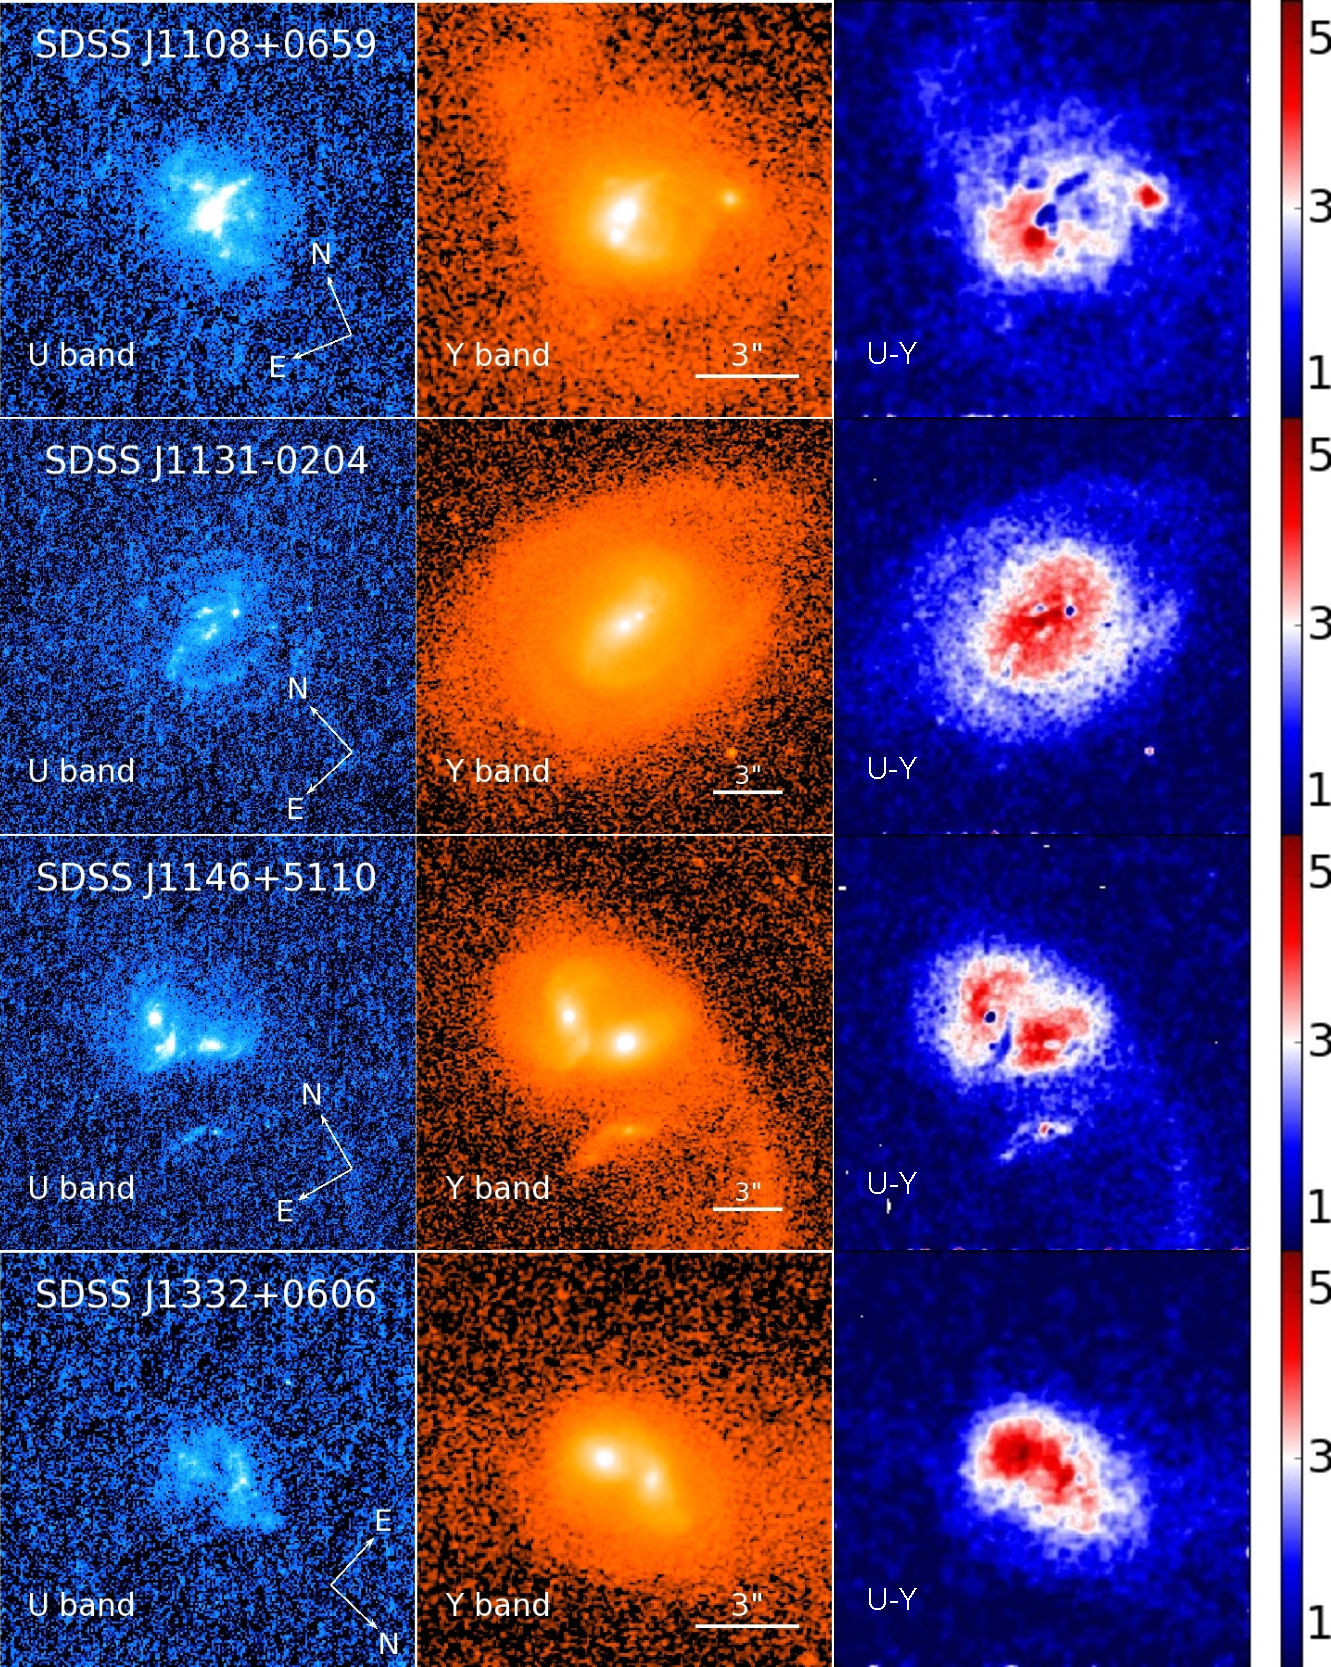
\includegraphics[width=0.95\textwidth]{../_demoResources/figs/zhihu/color_map.pdf}
\caption{
Images observed through U- and Y-band filters are shown in {\it left} and {\it middle} columns. 
The color maps are in the {\it right column}. 
The FOV and orientation of the images in each row are the same.
The compass and $3''$ scale bar are on the lower right corner of {\it left} and {\it middle} panels in each row.
}
\label{fig:cmp}
\end{center}
\end{figure*}



\begin{figure*}[!htpb]
\begin{center}
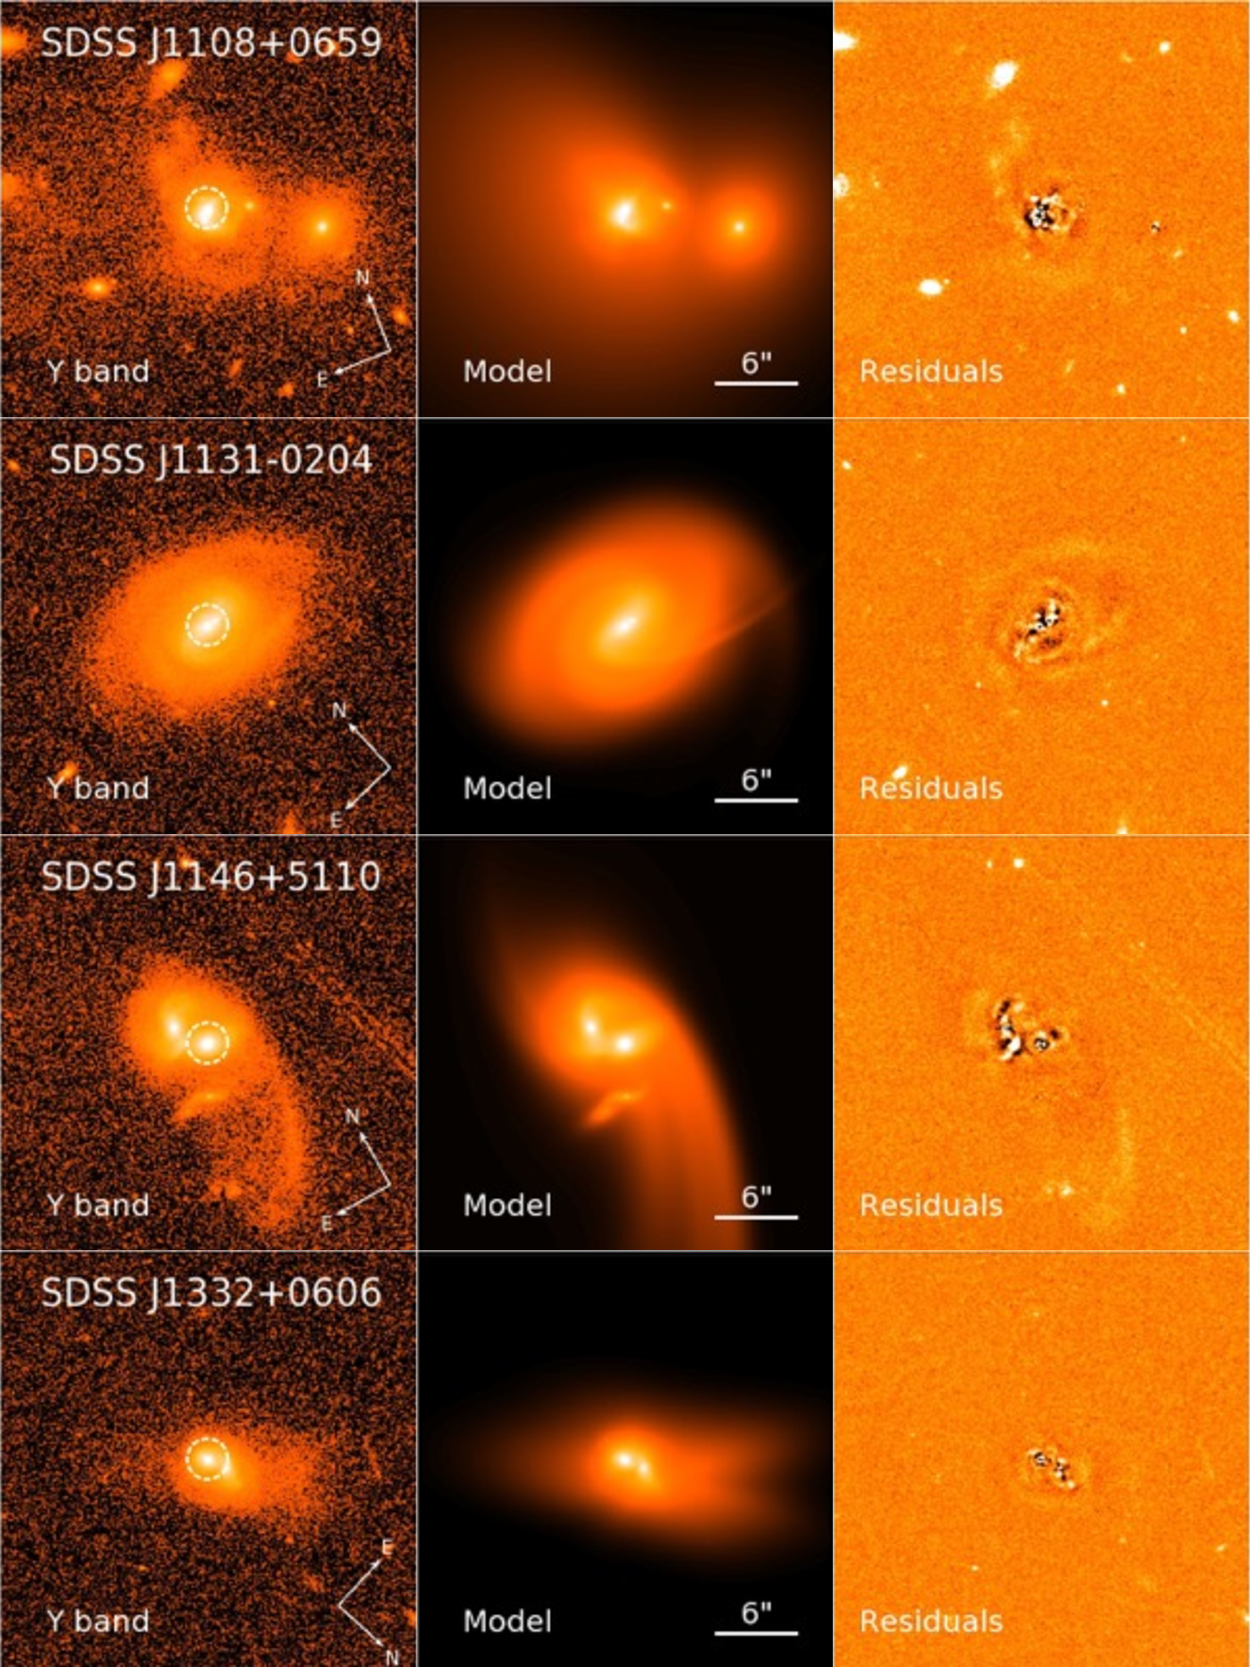
\includegraphics[width=0.95\textwidth]{../_demoResources/figs/zhihu/IR_galfit.pdf}
\caption{
Model fits of the \hst\ $Y$-band images of the four sources. 
{\it Left column} is the $Y$-band image of each target. 
The white dashed circles demonstrate the coverage of SDSS fibers ($3''$ in diameter). 
The compass of each image is shown in the lower right corner. 
{\it Middle column} is \galfit\ best fit of each target. 
The scale bar is shown in the lower-right corner. 
The FOVs of three panels in each row are the same. 
The pixel brightness scale is logarithmic in the first two columns. 
The residuals are show in {\it Right column}, where the pixel brightness scale is linear. 
We simultaneously fit the close companions of J1108 and J1146.
}
\label{fig:galfit}
\end{center}
\end{figure*}


\newsinglepage
\bibliography{../_demoResources/references/SimpleOneColumn/ref0}
\clearpage
\end{singlepage}

\end{document}
